% !TeX root = algorithmik.tex

\section{Elementares über Graphen}


\begin{definition}
    \index{Graph}
    \index{Endpunkte}
    \index{Parallelität}
    \index{Grad}
    
    Ein ungerichteter Graph ist ein Paar $G = (V,E)$, mit $V, E$ Mengen. $V$
    heißt Menge von Knoten, $E$ heißt Menge von Kanten. Außerdem gibt es eine
    Funktion $i: E \rightarrow \mathcal{P}(V)$ mit $\mathcal{P}(V) = 2^V$
    (Potenzmenge) und $0 < i(e) \leq 2$. $i$ gibt die Endpunkte einer Kante an.
    
    Ist $i(e) = \{ u, v \}$, so heißen $u, v$ Endpunkte von $e$. Ist $i(e_1)
    = i(e_2)$, so heißen $e_1, e_2$ parallel. Ist $|i(e)| = 1$, so heißt $e$
    Schleife.
    
    Der Grad eines Knotens $v$, $grad(v)$, ist die Anzahl der Kanten, für die
    $v$ Endpunkt ist, wobei Schleifen doppelt gezählt werden. Ist $grad(v)
    = 0$, so heißt $v$ isoliert.
    
    Ein Graph heißt endlich, wenn $V$ und $E$ endlich sind.
\end{definition}


\begin{beispiel}
    \qquad
    \vspace{2mm}
    
    \begin{minipage}{8cm}
        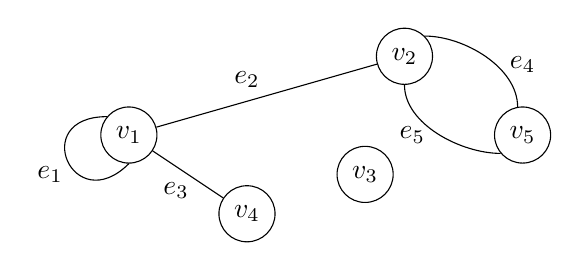
\begin{tikzpicture}
            \node (v4) at (2,0) [draw, shape=circle] {$v_4$};
            \node (v1) at (0.5,1) [draw, shape=circle] {$v_1$};
            \node (v3) at (3.5,0.5) [draw, shape=circle] {$v_3$};
            \node (v2) at (4,2) [draw, shape=circle] {$v_2$};
            \node (v5) at (5.5,1) [draw, shape=circle] {$v_5$};
            
            \draw(v4) -- (v1);
            \draw(v1) -- (v2);
            \draw(v1) -- (v1);
            \draw(v2.45) .. controls +(0:0.5) and +(90:0.5) .. (v5.100);
            \draw(v2.270) .. controls +(90:-0.5) and +(0:-0.5) .. (v5.220);
            \draw(v1.270) .. controls +(45:-1) and +(0:-1) .. (v1.140);
            
            \node (e1) at (-0.5, 0.5) { $e_1$ };
            \node (e2) at (2, 1.7) { $e_2$ };
            \node (e4) at (5.5, 1.9) { $e_4$ };
            \node (e5) at (4.1, 1) { $e_5$ };
            \node (e3) at (1.1, 0.3) { $e_3$ };
        \end{tikzpicture}
    \end{minipage}
    \begin{minipage}{5cm}   
    \begin{tabular}[t]{rl}
        $v_3$ & isoliert \\
        $e_4, e_5$ & parallel \\
        $e_1$ & Schleife \\
        $i(e_4) =$& $ \{ v_2, v_5 \} = i(e_5)$\\
        $grad(v_1) =$& $4$ \\
        $grad(v_2) =$& $3$ \\
    \end{tabular}
    \end{minipage}
\end{beispiel}


\begin{beispiel}
    Unendliche Graphen
    
    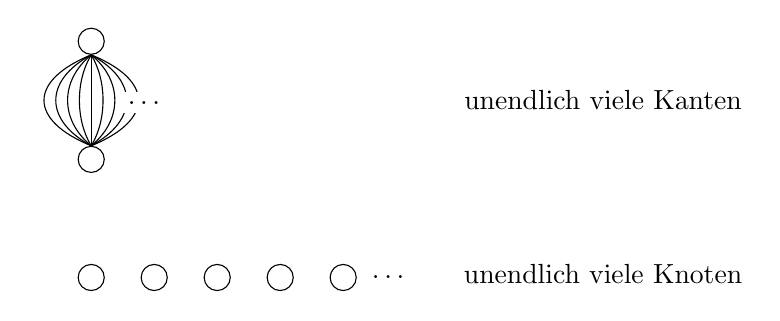
\begin{tikzpicture}
        \node (v1) at (0, 1.5) [draw, shape=circle] {};
        \node (v2) at (0, 0) [draw, shape=circle] {};
        
        \foreach \a in {-0.8, -0.6, -0.4, -0.2, 0, 0.2, 0.4, 0.6, 0.8}
            \draw (v1.south) .. controls (\a,1) and (\a, 0.5) .. (v2.north);
            
        \node (punkte) at (0.7, 0.72) [fill=white] {\dots};
        \node (bla) at (6.5, 0.76) {unendlich viele Kanten};
        
        \foreach \a in {0, 0.8, 1.6, 2.4, 3.2}
            \node at (\a, -1.5) [draw, shape=circle] {};
            
        \node (punkte2) at (3.8, -1.5) {\dots};
        \node (bla2) at (6.5, -1.45) {unendlich viele Knoten};
    \end{tikzpicture}
\end{beispiel}


\begin{bemerkung}
    In einem endlichen Graph ist die Anzahl der Knoten mit ungeradem Grad gerade.
\end{bemerkung}


\begin{beweis}
    Sei $V = \{ v_1, \dots, v_n \}$, dann ist $\sum_{i=1}^n grad(v_i) = 2 |E|$.
    Denn: starten wir mit $G = (V, \emptyset)$ und fügen die Kanten
    nacheinander ein, dann erhöht das Einfügen den Grad beider beteiligten
    Knoten um jeweils 1. Handelt es sich bei der Kante um eine Schleife, wir
    der Grad des Knotens um 2 erhöht.
    
    Seien o.E. $v_1 \dots v_j$ mit geradem Grad und $v_{j+1} \dots v_n$ mit
    ungeradem Grad. $\sum_{l=1}^j grad(v_l)$ ist eine gerade Zahl. Über alle
    Knoten summiert ergibt sich auch eine gerade Zahl $2|E|$.  $$ 2|E|
    = \sum_{i=1}^n grad(v_i) = \underbrace{\sum_{i=1}^j grad(v_i)}_{gerade}
    + \underbrace{\sum_{i=j+1}^n \overbrace{grad(v_i)}^{ungerade}}_{gerade} $$
    Damit $\sum_{i=j+1}^n grad(v_i)$ gerade ist, muss die Anzahl dieser
    ungeraden Knoten gerade sein.
\end{beweis}


\begin{definition}
    \index{Weg}
    \index{Schleife}
    
    Sei $G = (V,E)$ ein Graph. Sind $v_1, v_2$ die Endpunkte von $e$, so heißen
    $v_1, v_2$ benachbart. Ein Weg in G ist eine Folge von Kanten $e_1, e_2,
    \dots$, so dass gilt:
    \begin{enumerate}
        \item $\forall i$ gilt: $e_i, e_{i+1}$ haben einen gemeinsamen Endpunkt.
        \item ist $e_i$ keine Schleife und weder erste noch letzte Kante, so
            hat $e_i$ einen Knoten mit $e_{i-1}$ gemeinsam und den anderen mit
            $e_{i+1}$.
    \end{enumerate}
\end{definition}    


\begin{beispiel}
    \qquad
    \vspace{2mm}
    
    \begin{minipage}{4cm}
        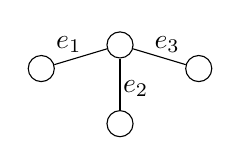
\begin{tikzpicture}
            \node (v1) at (0, -0.3) [draw, shape=circle] {};
            \node (v2) at (1, 0) [draw, shape=circle] {};
            \node (v3) at (2, -0.3) [draw, shape=circle] {};
            \node (v4) at (1, -1) [draw, shape=circle] {};
            
            \draw (v1) -- (v2);
            \draw (v2) -- (v3);
            \draw (v2) -- (v4);
            
            \node (l1) at (0.35, 0) {$e_1$};
            \node (l2) at (1.6, 0) {$e_3$};
            \node (l3) at (1.2, -0.55) {$e_2$};
            
        \end{tikzpicture}
    \end{minipage}
    \begin{minipage}{10cm}
        Ist $e_1, e_2, e_3$ ein Weg?
        
        \emph{1. ist erfüllt, 2. nicht $\Rightarrow$ kein Weg}
         
         $e_1, e_2, e_2, e_3$ ist ein Weg.
    \end{minipage}
\end{beispiel}


\begin{definition}
    Ein Weg wird auch folgendermaßen dargestellt:
    \vspace{2mm}
    
    \begin{center}
        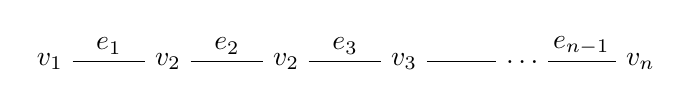
\begin{tikzpicture}
            \node (v1) at (0, 0) {$v_1$};
            \node (v2) at (1.5, 0) {$v_2$};
            \node (v22) at (3, 0) {$v_2$};
            \node (v3) at (4.5, 0) {$v_3$};
            \node (v4) at (6, 0) {$\dots$};
            \node (v5) at (7.5, 0) {$v_n$};
            
            \draw (v1) -- (v2);
            \draw (v2) -- (v22);
            \draw (v22) -- (v3);
            \draw (v3) -- (v4);
            \draw (v4) -- (v5);
            
            \node (l1) at (0.75, 0.2) {$e_1$};
            \node (l2) at (2.25, 0.2) {$e_2$};
            \node (l3) at (3.75, 0.2) {$e_3$};
            \node (l4) at (6.75, 0.2) {$e_{n-1}$};

        \end{tikzpicture}
    \end{center}
    
    In diesem Weg entspricht $e_2$ einer Schleife an $v_2$. Ist dieser
    abgebildete Weg endlich, so heißen $v_1$ Anfangspunkt und $v_n$ Endpunkt.
    Die Länge eines Weges ist gleich der Anzahl der Kanten, die er enthält.
    
    \index{Kreis}
    \index{Zyklus}
    \index{Kreis!einfach}
    \index{Weg!einfach}
    Ein Kreis (Zyklus) ist ein Weg, dessen Anfangspunkt und Endpunkt gleich
    sind. Ein Weg heißt einfach, wenn jeder Knoten höchstens einmal vorkommt. 
    
    Ein Kreis der Länge $\ne 2$ heißt einfach, wenn jeder Knoten außer Anfangs-
    und Endpunkt höchstens einmal vorkommt. 
    
    Ein Kreis der Länge 2 heißt einfach, wenn die beiden Kanten verschieden
    sind, und wenn jeder Knoten außer dem Start/Endpunkt höchstens einmal
    vorkommt und der Start/Endpunkt sonst nirgends.
\end{definition}

\begin{beispiel}
    \qquad
    \vspace{2mm}
    
    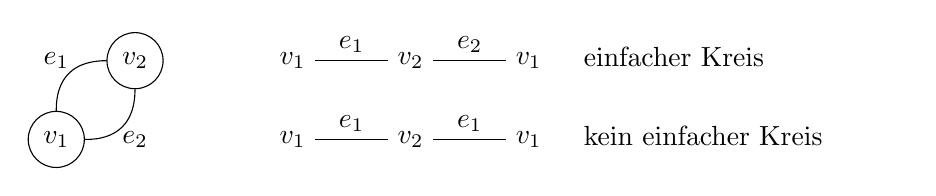
\begin{tikzpicture}
        \node (v1) at (0, 0) [draw, shape=circle] {$v_1$};
        \node (v2) at (1, 1) [draw, shape=circle] {$v_2$};
        
        \draw (v1) .. controls (up:0.5) and (up: 1) .. (v2);
        \draw (v1) .. controls (right:0.5) and (right: 1) .. (v2);
        
        \node (l1) at (0, 1) {$e_1$};
        \node (l2) at (1, 0) {$e_2$};
    
        \node (v1a) at (3, 0) {$v_1$};
        \node (v2a) at (4.5, 0) {$v_2$};
        \node (v1b) at (6, 0) {$v_1$};
        
        \draw (v1a) -- (v2a);
        \draw (v2a) -- (v1b);
        
        \node (l3) at (3.75, 0.2) {$e_1$};
        \node (l4) at (5.25, 0.2) {$e_1$};
        
        \node (v1c) at (3, 1) {$v_1$};
        \node (v2b) at (4.5, 1) {$v_2$};
        \node (v1d) at (6, 1) {$v_1$};
        
        \draw (v1c) -- (v2b);
        \draw (v2b) -- (v1d);
        
        \node (l5) at (3.75, 1.2) {$e_1$};
        \node (l6) at (5.25, 1.2) {$e_2$};
        
        \node[text width=4cm] (l7) at (8.7, 1.05) {einfacher Kreis};
        \node[text width=4cm] (l8) at (8.7, 0.05) {kein einfacher Kreis};
    \end{tikzpicture}
\end{beispiel}


\begin{definition}
    \index{Graph!zusammenhängend}
    
    Ein Graph $G = (V, E)$ heißt zusammenhängend, wenn es zwischen je zwei
    Knoten in $V$ einen Weg gibt, der sie verbindet, d.h. einer der Knoten ist
    Anfangspunkt und einer ist Endpunkt. 
    
    Es gibt für jeden Knoten $v$ der Menge $V$ einen Weg zu $v$ der Länge $0$.
\end{definition}


\begin{definition}
    \index{Separationspunkt}
    \index{Graph!separabel}
    
    Sei $G = (V, E)$ ein zusammenhängender Graph. Ein Knoten $a \in V$ heißt
    Separationspunkt, wenn es Knoten $u$ und $v$ gibt, so dass jeder Weg
    zwischen $u$ und $v$ über den Knoten $a$ führt.
    
    Hat $G$ einen Separationspunkt, so heißt der Graph separabel, ansonsten
    unseparabel. Eine Kante $e$ heißt Brücke, wenn es zwei Knoten $u, v$ gibt,
    so dass jeder Weg von $u$ nach $v$ über die Kante $e$ läuft.
\end{definition}


\begin{definition}
    \index{Graph!bipartit}
    
    Ein Graph $G = (V, E)$ ohne Schleifen heißt bipartit (zweigeteilt), wenn es
    Mengen $V_1, V_2 \subseteq V$ gibt, so dass für jede Kante gilt: ein
    Endpunkt liegt in $V_1$, der andere in $V_2$.
\end{definition}


\begin{beispiel}
    \qquad
    \vspace{2mm}
    
    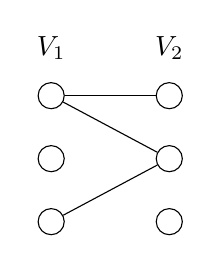
\begin{tikzpicture}
        \node (V1) at (0, 2.2) {$V_1$};
        \node (V2) at (1.5, 2.2) {$V_2$};
        
        \node (v1) at (0, 0) [draw, shape=circle] {};
        \node (v2) at (0, 0.8) [draw, shape=circle] {};
        \node (v3) at (0, 1.6) [draw, shape=circle] {};
        
        \node (v4) at (1.5, 0) [draw, shape=circle] {};
        \node (v5) at (1.5, 0.8) [draw, shape=circle] {};
        \node (v6) at (1.5, 1.6) [draw, shape=circle] {};
        
        \draw (v3) -- (v6);
        \draw (v1) -- (v5);
        \draw (v3) -- (v5);
    \end{tikzpicture}
\end{beispiel}


\begin{definition}
    \index{Graph!gerichtet}
    \index{Parallelität}
    \index{Schleife}
    \index{Ausgrad}
    \index{Ingrad}

    Ein gerichteter Graph ist ein Paar $G = (V, E)$ mit der Menge der Knoten
    $V$, der Menge der Kanten $E$ und der Abbildung $i: E \rightarrow V \times
    V$. Ist $i(e) = (u, v)$, so heißt $u$ Anfangspunkt und $v$ Endpunkt von
    $e$.
    
    Ist $i(e_1) = i(e_2)$, so heißen $e_1$ und $e_2$ parallel. Ist $u \ne v$
    und $i(e_1) = (u, v)$ und $i(e_2) = (v, u)$, so heißen $e_1, e_2$
    antiparallel. Ist $i(e) = (v, v)$, so heißt $e$ Schleife.
    
    \begin{itemize}
        \item $g_{out}(u)$: Anzahl der Kanten, die $u$ als Startpunkt haben. (Ausgrad)
        \item $g_{in}(u)$: Anzahl der Kanten, die $u$ als Endpunkt haben. (Ingrad)
    \end{itemize}
\end{definition}


\begin{bemerkung}
    Für jeden gerichteten Graph mit $V = \{ v_1, v_2, \dots, v_n \}$ gilt:
    $$\sum_{i=1}^n g_{in}(v_i) = \sum_{i=1}^n g_{out}(v_i)$$
    Begründung: Starte mit dem Graph ohne Kanten. Füge nacheinander alle Kanten
    ein. Das Einfügen einer Kante $e$ trägt zur Summe auf der linken Seite und
    zur Summe auf der rechten Seite je $1$ bei.
\end{bemerkung}


\begin{definition}
    \index{Weg!gerichtet}
    \index{Kreis!gerichtet}
    \index{Kreis!einfach}
    \index{Weg!einfach}
    
    Ein gerichteter Weg ist eine Folge von Kanten $e_1, e_2, \dots, e_n$, so
    dass $\forall i \in \{ 1, \dots, n-1 \}$ gilt: der Endpunkt von $e_i$ ist
    der Anfangspunkt von $e_{i+1}$.
    
    Ein endlicher gerichteter Weg heißt Kreis (Zyklus), wenn Anfangspunkt und
    Endpunkt übereinstimmen. Ein einfacher Weg ist ein Weg, in dem jeder Knoten
    nur einmal vorkommt.
    
    Ein gerichteter Kreis heißt einfach, wenn kein Knoten außer Anfangs- und
    Endpunkt mehrfach vorkommt.
\end{definition}


\begin{definition}
    \index{Graph!einfach}

    Ein Graph (gerichtet oder ungerichtet) heißt einfach, wenn er keine
    parallelen Kanten besitzt.
\end{definition}


\begin{definition}
    \index{Graph!kreisfrei}
    \index{Baum}
    
    Ein ungerichteter Graph $G$ heißt Kreisfrei, wenn er keinen einfachen Kreis
    enthält. $G$ heißt Baum, wenn $G$ kreisfrei und zusammenhängend ist.
\end{definition}


\begin{definition}
    \index{Wurzel}
    \index{Baum!gerichtet}

    Sei $G = (V, E)$ ein gerichteter Graph. Ein Knoten $v \in V$ heißt Wurzel,
    wenn von $v$ alle Knoten $w \in V$ aus $v$ erreichbar sind, d.h. $\forall
    w$  existiert ein gerichteter Weg von $v$ nach $w$. $G$ heißt gerichteter
    Baum, wenn $G$ eine Wurzel besitzt und der zugrundeliegende ungerichtete
    Graph ein Baum ist.
\end{definition}


\begin{bemerkung}
    $G$ ist gerichteter Baum genau dann wenn
    \begin{enumerate}
        \item der zugrundeliegende ungerichtete Graph kreisfrei ist,
        \item einer der Knoten $r \in V$ die Bedingung $g_{in}(r) = 0$ erfüllt,
        \item alle anderen Knoten $v \in V$ die Bedingung $g_{in}(v) = 1$ erfüllen.
    \end{enumerate}
\end{bemerkung}


\begin{definition}
    \index{Knoten!übergeordnet}
    \index{Graph!übergeordnet}

    Sei $G$ ein gerichteter Graph, $v_1, v_2 \in V$. Ein Knoten $v \in V$ heißt
    \emph{übergeordnet} für $v_1, v_2$, wenn es einen Weg von $v$ nach $v_1$
    und $v_2$ gibt.
    
    $G$ heißt übergeordnet, wenn es für je zwei Knoten $v_1, v_2$ einen Knoten
    $v$ gibt, der für sie übergeordnet ist.
    
    \begin{enumerate}
        \item Bäume (endlich oder unendlich) sind übergeordnet.
        \item $\bigcirc \leftarrow \bigcirc \leftarrow \bigcirc \leftarrow
            \dots$ ist übergeordnet.
        \item Jeder Graph mit Wurzel ist übergeordnet.
    \end{enumerate}
\end{definition}


\begin{bemerkung}
    Jeder endliche übergeordnete Graph hat eine Wurzel.
\end{bemerkung}


\begin{definition}
    \index{Quelle}
    \index{Senke}

    Sei $G = (V,E)$ ein gerichteter Graph. Ein Knoten $v \in V$ heißt Quelle,
    wenn $g_{in}(v) = 0$, und Senke, wenn $g_{out}(v) = 0$.

\end{definition}
